% \documentclass[handout]{beamer}
\documentclass[presentation]{beamer}
\usepackage[utf8]{inputenc}
\usepackage{amsmath, pdfpages, pdflscape, lscape, color, listings, hyperref, amssymb, graphicx, textcomp,varioref, afterpage, subcaption, float, bm, tikz, colortbl, caption}




\setbeamertemplate{blocks}[rounded][shadow=false]


\usefonttheme[onlysmall]{structurebold}
% Use a bold face title font
\setbeamerfont{title}{series=\bfseries}
\setbeamerfont{frametitle}{series=\bfseries}

% This is not created yet, but should be...
%\usecolortheme{simula}

% Suppress navigation symbols
\setbeamertemplate{navigation symbols}{}

\definecolor{myred}{RGB}{190,0,0}

\definecolor{logogrey}{HTML}{426E86}
\definecolor{logored}{HTML}{E50000}
\definecolor{logoyellow}{HTML}{F9BA32}


\definecolor{listingsstringcolor}{rgb}{0,0.5,0}
\definecolor{listingskeywordcolor}{rgb}{0.5,0.5,0.0}
\definecolor{listingsbasiccolor}{rgb}{0.0,0.0,0.0}
% \definecolor{listingskeywordcolor}{rgb}{0.0,0.0,0.7}
%\definecolor{listingsnumbercolor}{rgb}{0.6,0.6,0.6}
\definecolor{listingsnumbercolor}{rgb}{0.35,0.35,0.35}
\definecolor{listingscommentcolor}{rgb}{0.4,0.4,0.4}
\definecolor{listingsbackgroundcolor}{rgb}{0.975,0.975,0.975}
\definecolor{listingsrulecolor}{rgb}{0.86,0.86,0.86}
\definecolor{listingsidentifiercolor}{rgb}{0.0,0.0,0.0}
\definecolor{listingsclasscolor}{rgb}{0.5,0.0,0.5}
\definecolor{listingsmembercolor}{rgb}{0.5,0.0,0.0}
\definecolor{listingsdirectivecolor}{rgb}{0.0,0.0,0.5}
% \definecolor{listingsvariablecolor}{rgb}{0.5,0.0,0.5}
\definecolor{pyoutbackground}{rgb}{1.0, 1.0, 1.0}
\definecolor{pyoutrule}{rgb}{.25882353,  0.64705882,  0.96078431}

\RequirePackage{iftex}
\newcommand{\listingsfont}{\ttfamily}
\ifxetex
  \usepackage{fontspec}
  \newfontfamily\listingsfontfamily[Scale=0.85]{Noto Mono}
  \renewcommand{\listingsfont}{\listingsfontfamily}
\fi

\lstset {
    language=Python,
    morekeywords={as, assert, with, yield, self},
    %backgroundcolor=\color{listingsbackgroundcolor},
    breakatwhitespace=true,         % sets if automatic breaks should only happen at whitespace
    breaklines=false,                 % sets automatic line breaking
    numbers=none,                    % where to put the line-numbers; possible values are (none, left, right)
    numbersep=18pt,                   % how far the line-numbers are from the code
    frame=none,                    % adds a frame around the code
    framexleftmargin=7pt,
    framexrightmargin=7pt,
    framextopmargin=0pt,
    framexbottommargin=0pt,
    xleftmargin=18pt,
    xrightmargin=18pt,
    rulecolor=\color{listingsrulecolor},
    tabsize=4,                       % sets default tabsize to 2 spaces
    literate={-}{{\textendash}}1 {å}{{\aa}}1 {æ}{{\ae}}1 {ø}{{\oslash}}1,
    showstringspaces=false,
    captionpos=b,
    escapeinside={(*@}{@*)},
    %columns=fixed
    basicstyle=\color{listingsbasiccolor}\footnotesize\listingsfont,
    keywordstyle=\color{listingskeywordcolor}\footnotesize\listingsfont,
%    directivestyle=\color{listingsdirectivecolor}\footnotesize\listingsfont,
    stringstyle=\color{listingsstringcolor}\footnotesize\listingsfont,
    commentstyle=\color{listingscommentcolor}\footnotesize\listingsfont,
    numberstyle=\color{listingsnumbercolor}\footnotesize\listingsfont,
    identifierstyle=\color{listingsidentifiercolor}\footnotesize\listingsfont,
    keywordstyle=[2]{\color{listingsclasscolor}\footnotesize\listingsfont},
    keywordstyle=[3]{\color{listingsmembercolor}\footnotesize\listingsfont},
    keywordstyle=[4]{\color{listingsdirectivecolor}\footnotesize\listingsfont},
}



\definecolor{keywords}{RGB}{255,0,90}
\definecolor{comments}{RGB}{0,0,113}
\definecolor{red}{RGB}{160,0,0}
\definecolor{green}{RGB}{0,150,0}


\setbeamercolor{title}{fg=logored}
\setbeamercolor{frametitle}{fg=black!65!white,bg=white}
\setbeamercolor{normal text}{fg=black!75!white,bg=white}
\setbeamercolor{structure}{fg=black,bg=white}






\newcommand{\fullimage}[2]{
    \begin{tikzpicture}[remember picture, overlay]
      \node[anchor = center] (image) at (current page.center) {\includegraphics[scale=#2]{#1}};
    \end{tikzpicture}
}


\graphicspath{{./figures/}}




\begin{document}

% \maketitle

% \begin{frame}
%    \begin{tikzpicture}[remember picture, overlay]
%      \node[anchor = center, opacity=.25] (image) at (current page.center) {\includegraphics[scale=0.25]{chaospy_logo.jpg}};
%    \end{tikzpicture}
%
% \begin{center}
%     \textbf{ \color{myred} \Large Chaospy: \\ \vspace{1mm} A modular implementation of polynomial\\ \vspace{1mm} chaos expansions and Monte Carlo methods}
% \end{center}
% \begin{center}
%      \large \vspace{5mm} Simen Tennøe\\ \vspace{5mm}\footnotesize Supervisors:\\ \vspace{0.5mm} Jonathan Feinberg, Hans Petter Langtangen, Gaute Einevoll and Geir Halnes
% \end{center}
%
% \begin{center}
%     \small University of Oslo, CINPLA
% \end{center}
% %\includegraphics[width=\textwidth]{chaospy_logo.jpg}
%
% \end{frame}



\begin{frame}
    \fullimage{network.jpeg}{0.65}
\end{frame}



\begin{frame}%{\color{myred} Beregningsorientert nevrovitenskap}
\begin{center}
\vspace{-40mm}
    \textbf{\color{myred}\LARGE Beregningsorientert nevrovitenskap}
    \vspace{3mm}

    Simen Tennøe
\end{center}

 \begin{tikzpicture}[remember picture,overlay]
    \node [xshift=0\paperwidth, yshift=-0.1\paperheight] at (current page.center)
          {
\includegraphics[width = 0.8\paperheight ]{logo-only.png}};
  \end{tikzpicture}

  % \begin{tikzpicture}[remember picture,overlay]
  %   \node [xshift=1.35cm,yshift=0.55cm] at (current page.south west)
  %         {
\includegraphics[width = 0.3\paperwidth ]{cinpla.png}};
  % \end{tikzpicture}

      %  \large \vspace{8mm} Simen Tennøe  - \small University of Oslo, CINPLA

\end{frame}



\begin{frame}
    \fullimage{galaxy.jpg}{0.2}
\end{frame}



\begin{frame}[fragile]{}
    \begin{tikzpicture}[remember picture, overlay, font=\sffamily]
      \node [align=left, xshift=-0.4\textwidth,yshift=0.25\textwidth] (image3) at (current page.center)
            {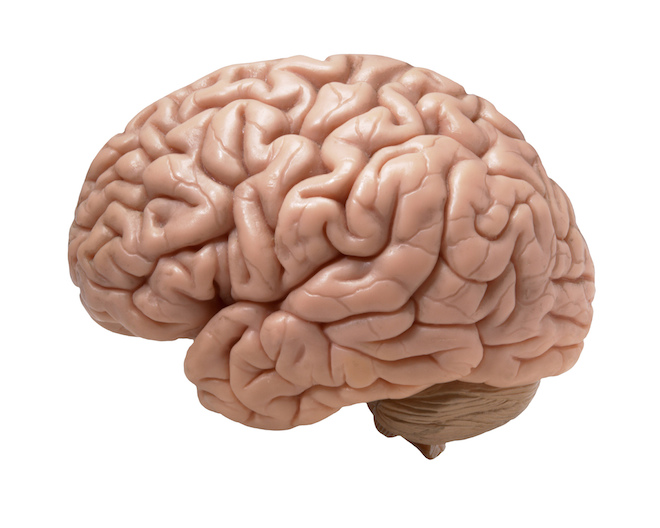
\includegraphics[width = 0.2\textwidth]{brain.jpg}};
      \node[align=left] at (image3.east) {\hspace{6cm} \bf Grunnlegende nevrovitenskap};
    \end{tikzpicture}

  \pause

  \begin{tikzpicture}[remember picture, overlay, font=\sffamily]
  \node [align=left, xshift=-0.2\textwidth,yshift=0\textwidth] (image1) at (current page.center)
      {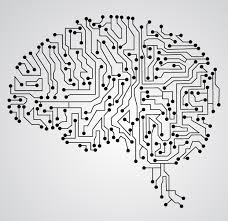
\includegraphics[width = 0.2\textwidth]{brain_circuits.jpg}};
  \node[align=left] at (image1.east) {\hspace{7.5cm} \bf Beregningsorientert nevrovitenskap};
  \end{tikzpicture}

\pause


    \begin{tikzpicture}[remember picture, overlay, font=\sffamily]
      \node [align=left, xshift=0\textwidth,yshift=-0.25\textwidth] (image2) at (current page.center)
            {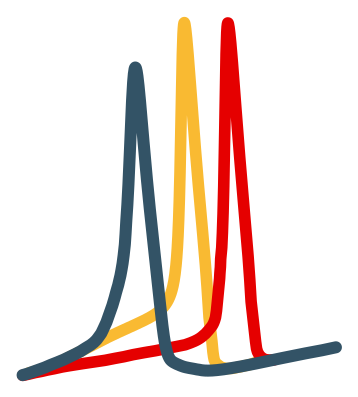
\includegraphics[width = 0.2\textwidth]{logo_small.png}};
      \node[align=left] at (image2.east) {\hspace{4.75cm} \bf Usikkerhet i nevrovitenskap};
    \end{tikzpicture}

\end{frame}














\begin{frame}[fragile]{}
    \begin{tikzpicture}[remember picture, overlay, font=\sffamily]
      \node [align=left, xshift=-0.4\textwidth,yshift=0.25\textwidth] (image3) at (current page.center)
            {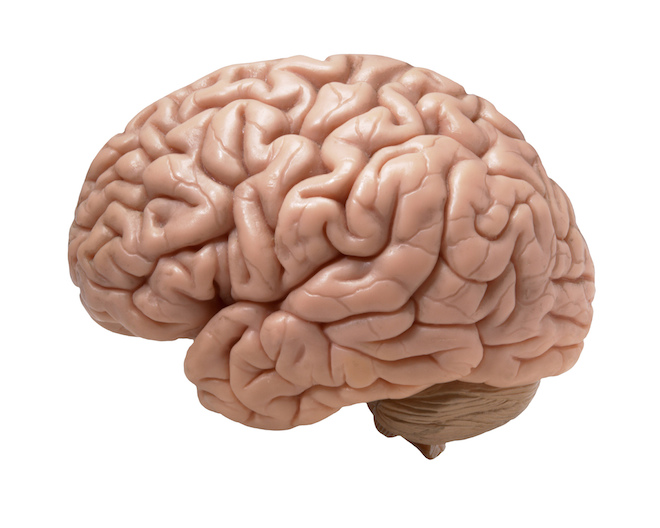
\includegraphics[width = 0.2\textwidth]{brain.jpg}};
      \node[align=left] at (image3.east) {\hspace{6cm} \bf Grunnlegende nevrovitenskap};
    \end{tikzpicture}

  \begin{tikzpicture}[remember picture, overlay, font=\sffamily]
  \node [align=left, opacity=0.35, xshift=-0.2\textwidth,yshift=0\textwidth] (image1) at (current page.center)
      {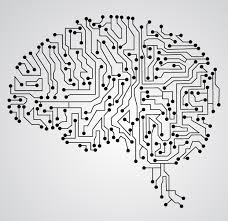
\includegraphics[width = 0.2\textwidth]{brain_circuits.jpg}};
  \node[align=left, opacity=0.35] at (image1.east) {\hspace{7.5cm} \bf Beregningsorientert nevrovitenskap};
  \end{tikzpicture}


    \begin{tikzpicture}[remember picture, overlay, font=\sffamily]
      \node [align=left, opacity=0.35, xshift=0\textwidth,yshift=-0.25\textwidth] (image2) at (current page.center)
            {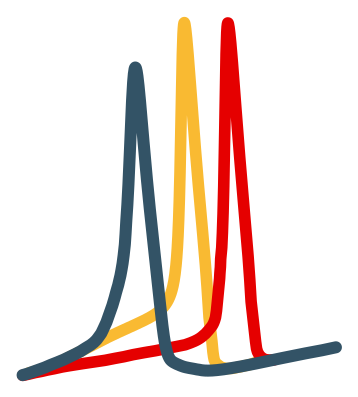
\includegraphics[width = 0.2\textwidth]{logo_small.png}};
      \node[align=left, opacity=0.35] at (image2.east) {\hspace{4cm} \bf Usikkerhetsberegninger};
    \end{tikzpicture}
\end{frame}


% \begin{frame}{Nevrovitenskap er studiet hjernen og nervesystemet}
%    \begin{figure}
%        {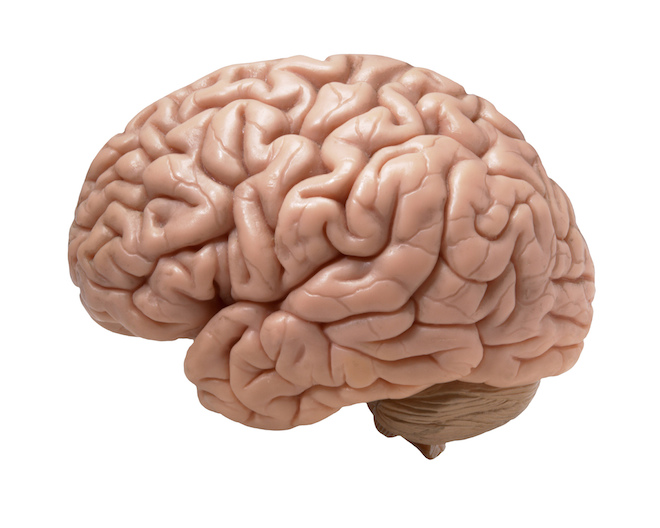
\includegraphics[width=1\textwidth]{brain.jpg}}
% \end{figure}
% \end{frame}

\begin{frame}
    \fullimage{brain.jpg}{2}
\end{frame}

% \begin{frame}{Hjerneceller (nevroner) kommuniserer via elektriske signaler}
%    \begin{figure}
%        {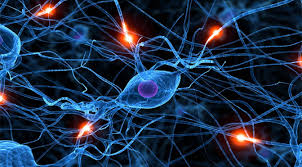
\includegraphics[width=0.9\textwidth]{network.jpeg}}
% \end{figure}
% \end{frame}

\begin{frame}
    \fullimage{network.jpeg}{0.65}
\end{frame}

% \begin{frame}{Nevroner fungerer som små batterier}
%     \vspace{-0.5cm}
%    \begin{figure}
%        {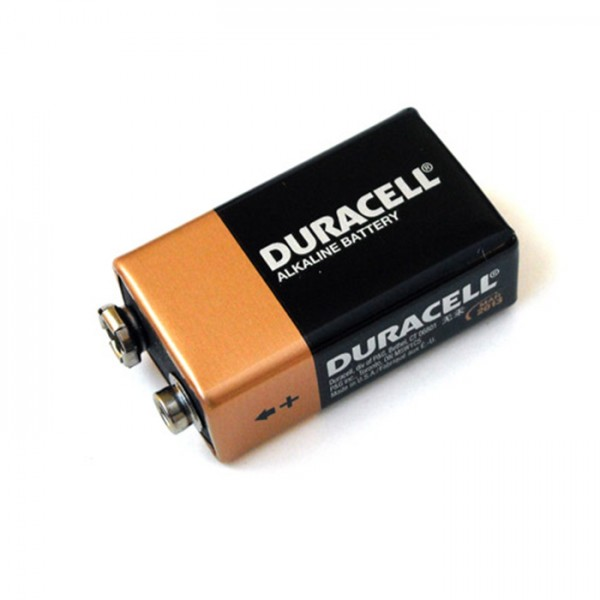
\includegraphics[width=0.4\textwidth]{battery.jpg}}
% \end{figure}
% \end{frame}


\begin{frame}
   \begin{figure}
       \only<1>{\fullimage{neuron2.png}{0.7}}
       \only<2>{\fullimage{neuron2_soma.png}{0.7}}
       \only<3>{\fullimage{neuron2_axon.png}{0.7}}
       \only<4>{\fullimage{neuron2_axon2.png}{0.7}}
    %    \only<5>{\fullimage{neuron2_dend.png}{0.7}}
\end{figure}
\end{frame}

\begin{frame}
    \fullimage{battery.jpg}{0.4}
\end{frame}

\begin{frame}{\color<-2>{white}Forskjellig konsentrasjon av positive og negative ioner (elektriske ladninger) setter opp ett elektrisk felt}
\vspace{-5mm}
   \begin{figure}
        \only<1>{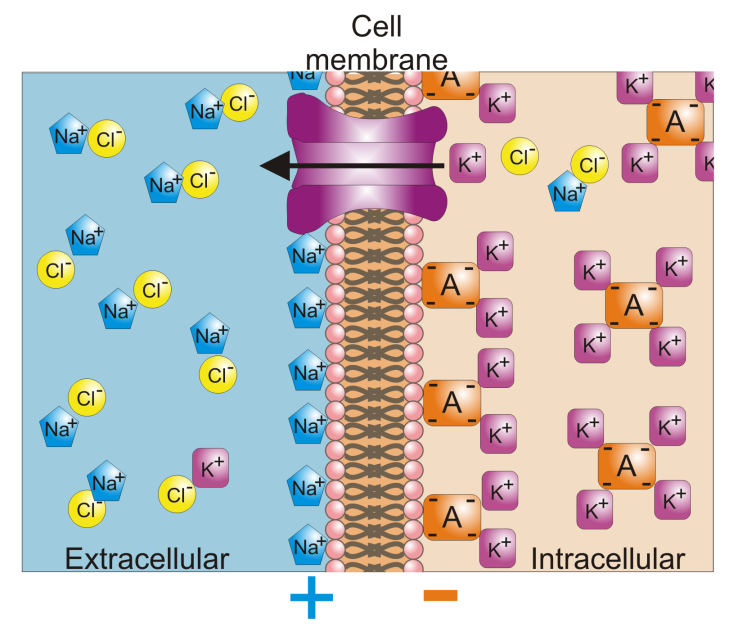
\includegraphics[width=1\textwidth]{membrane.png}}
        \only<2>{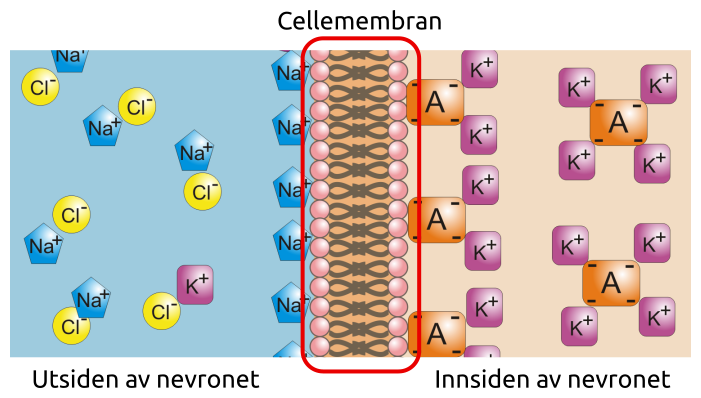
\includegraphics[width=1\textwidth]{membrane_focus.png}}
        % \only<3>{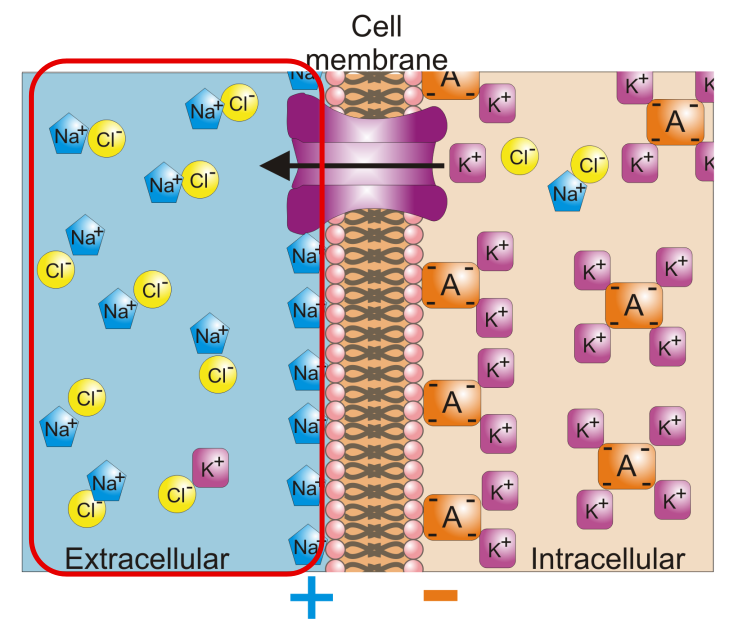
\includegraphics[width=0.8\textwidth]{membrane_out.png}}
        % \only<4>{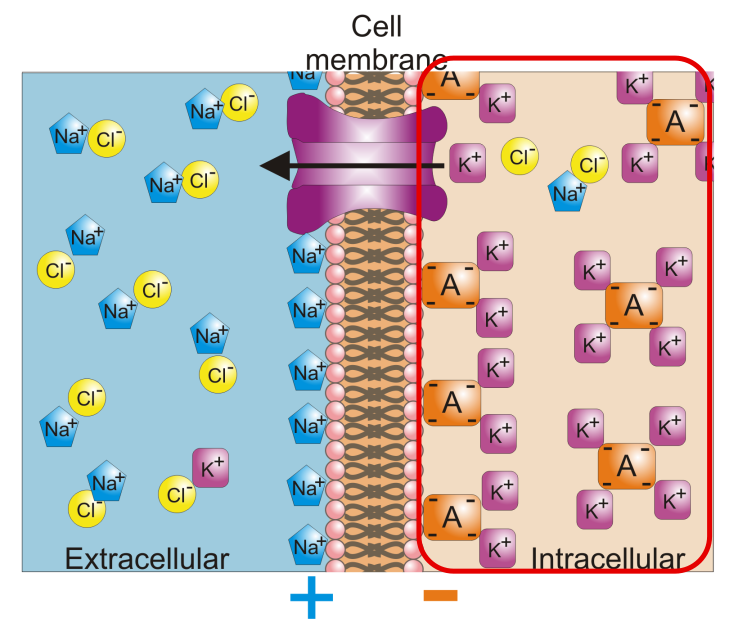
\includegraphics[width=0.8\textwidth]{membrane_in.png}}
        \only<3>{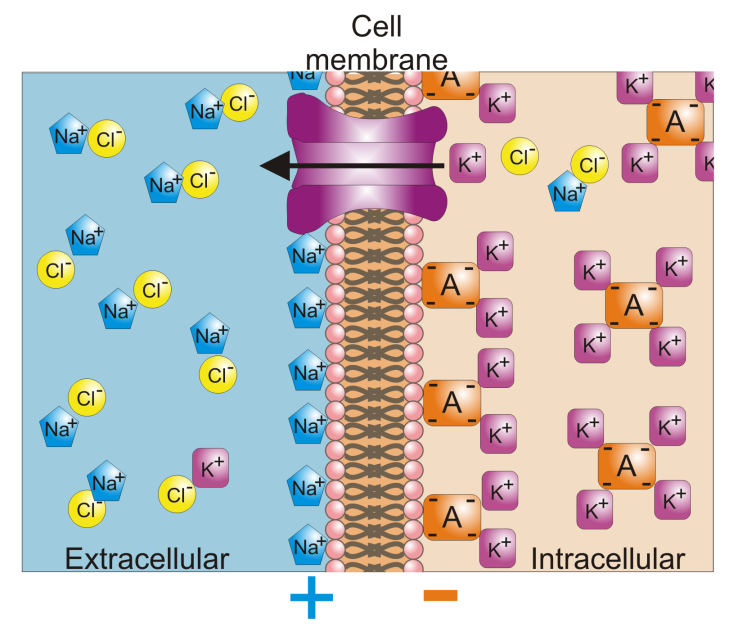
\includegraphics[width=1\textwidth]{membrane.png}}
        \only<4>{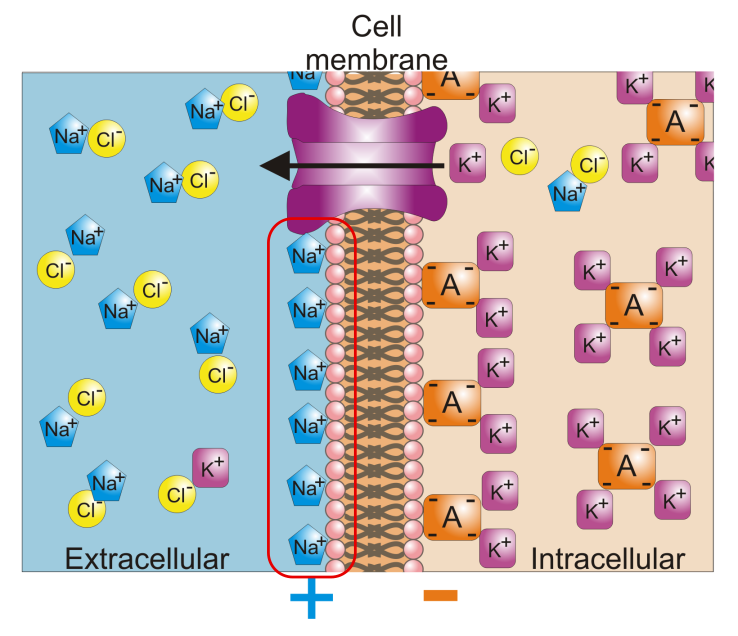
\includegraphics[width=1\textwidth]{membraneNa.png}}
        \only<5>{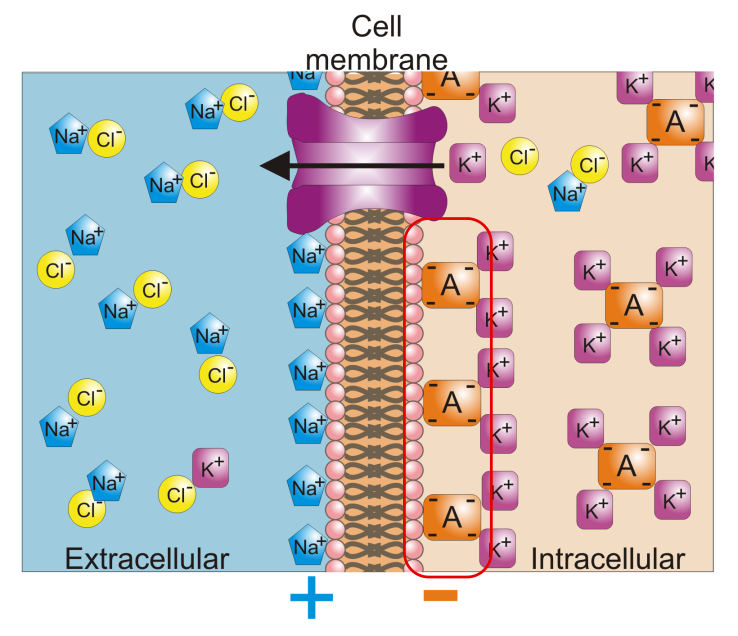
\includegraphics[width=1\textwidth]{membraneA.png}}
\end{figure}
\end{frame}


\begin{frame}{Ione pumper flytter ioner over cellemembranen}
   \begin{figure}
       {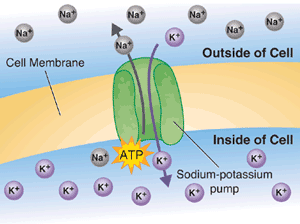
\includegraphics[width=0.9\textwidth]{ion_pump.png}}
\end{figure}
\end{frame}



\begin{frame}{Ione kanaler åpnes og slipper raskt ut ioner}
   \begin{figure}
       {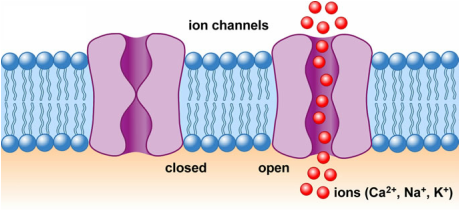
\includegraphics[width=1\textwidth]{ion_channel.png}}
\end{figure}
\end{frame}

% \begin{frame}{Signalene som sendes kalles aksjonspotensialer og er kortvarige forandringer i det elektriske potensialet}
%    \begin{figure}
%        {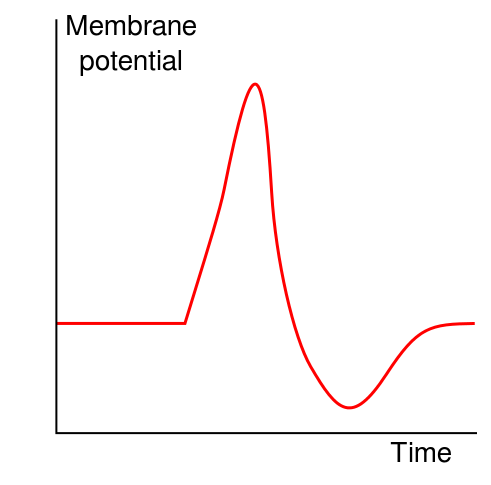
\includegraphics[width=0.7\textwidth]{ap.png}}
% \end{figure}
% \end{frame}

\begin{frame}
    \fullimage{ap.png}{0.5}
\end{frame}


%
% \begin{frame}{Signaler sendes mellom nevroner i nettverk som gjør... noe}
%    \begin{figure}
%        {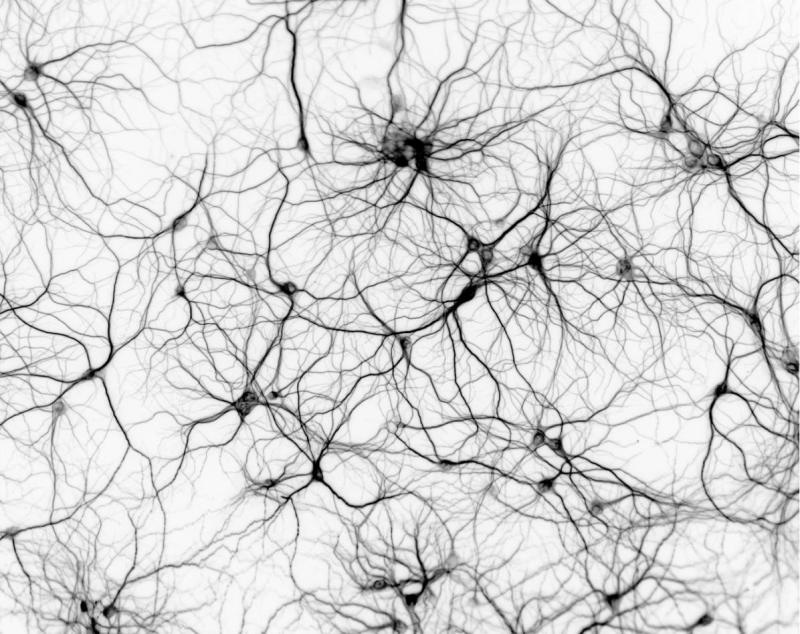
\includegraphics[width=0.8\textwidth]{network2.jpg}}
% \end{figure}
% \end{frame}

\begin{frame}
    \fullimage{network2.jpg}{0.5}
\end{frame}

\begin{frame}{}
    \begin{columns}
    \begin{column}{0.5\textwidth}
        \begin{center}
        \begin{figure}
            \only<1->{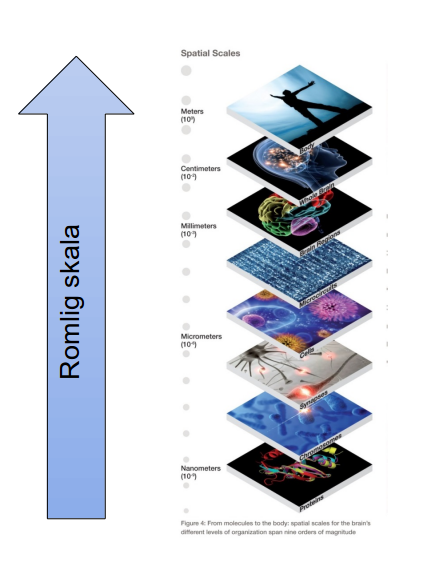
\includegraphics[width=1\textwidth]{romlig.png}}
     \end{figure}
    \end{center}
    \end{column}
    \begin{column}{0.5\textwidth}  %%<--- here
        \begin{center}
                \only<2>{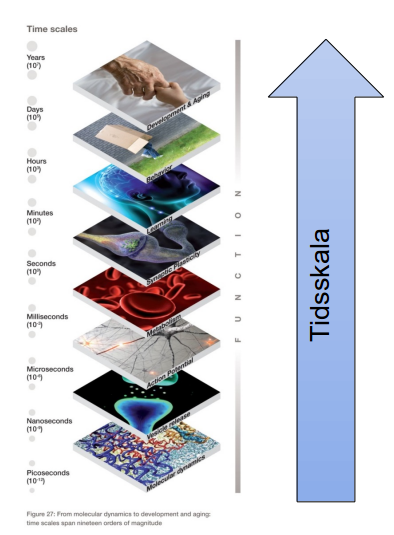
\includegraphics[width=1\textwidth]{tid.png}}
         \end{center}
    \end{column}
    \end{columns}
\end{frame}



% \begin{frame}{Analyse av store mengder data er og en utfordring}
%
%     Vi har data fra hundrevis av elektroder i hjernen
%     \begin{figure}
%             {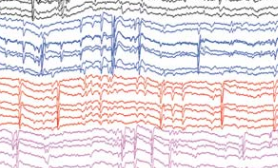
\includegraphics[width=1\textwidth]{analyse.png}}
%      \end{figure}
% \end{frame}

% \begin{frame}
%     \fullimage{analyse.png}{1.7}
% \end{frame}

\begin{frame}[fragile]{}
    \begin{tikzpicture}[remember picture, overlay, font=\sffamily]
      \node [align=left, opacity=0.35, xshift=-0.4\textwidth,yshift=0.25\textwidth] (image3) at (current page.center)
            {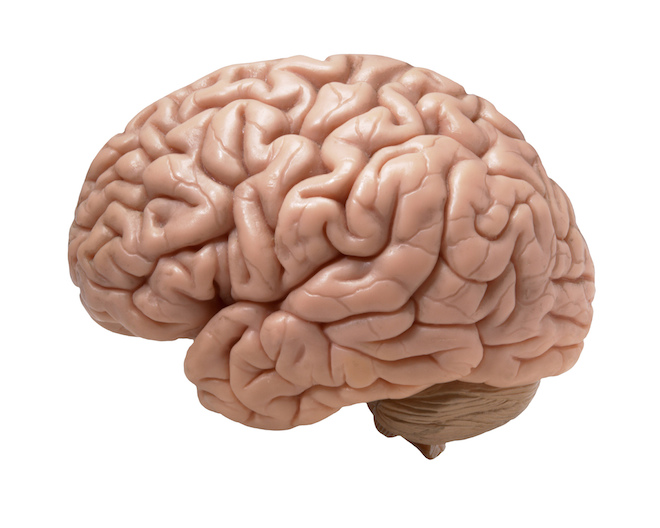
\includegraphics[width = 0.2\textwidth]{brain.jpg}};
      \node[align=left, opacity=0.35] at (image3.east) {\hspace{6cm} \bf Grunnlegende nevrovitenskap};
    \end{tikzpicture}

  \begin{tikzpicture}[remember picture, overlay, font=\sffamily]
  \node [align=left, xshift=-0.2\textwidth,yshift=0\textwidth] (image1) at (current page.center)
      {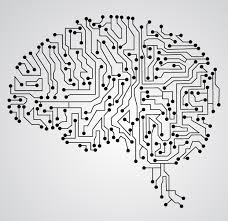
\includegraphics[width = 0.2\textwidth]{brain_circuits.jpg}};
  \node[align=left] at (image1.east) {\hspace{7.5cm} \bf Beregningsorientert nevrovitenskap};
  \end{tikzpicture}


    \begin{tikzpicture}[remember picture, overlay, font=\sffamily]
      \node [align=left, opacity=0.35, xshift=0\textwidth,yshift=-0.25\textwidth] (image2) at (current page.center)
            {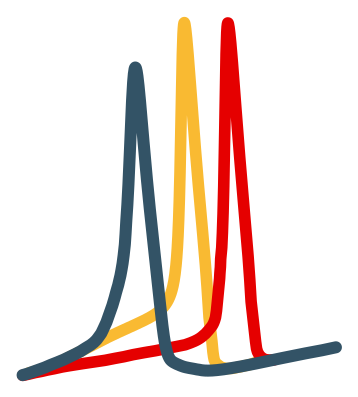
\includegraphics[width = 0.2\textwidth]{logo_small.png}};
      \node[align=left, opacity=0.35] at (image2.east) {\hspace{4cm} \bf Usikkerhetsberegninger};
    \end{tikzpicture}
\end{frame}



\begin{frame}{Ett nevron kan modeleres som en elektrisk krets}
    \begin{overlayarea}{\textwidth}{\textheight}

   \begin{figure}
       \only<1>{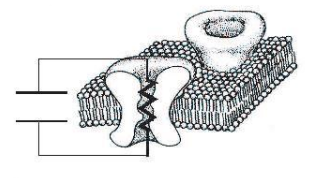
\includegraphics[width=1\textwidth]{circuit1_1.png}}
       \only<2>{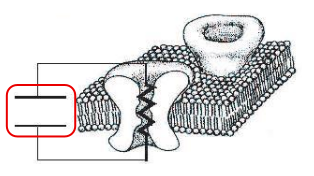
\includegraphics[width=1\textwidth]{circuit1_2.png}}
       \only<3>{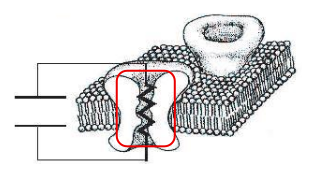
\includegraphics[width=1\textwidth]{circuit1_3.png}}
\end{figure}
\end{overlayarea}
\end{frame}


\begin{frame}{Ett nevron kan modeleres som en elektrisk krets}
    \begin{columns}
    \begin{column}{0.5\textwidth}
        \begin{center}
        \begin{figure}
            {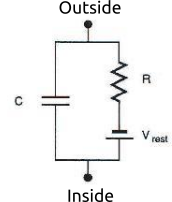
\includegraphics[width=1\textwidth]{circuit2.png}}
     \end{figure}
    \end{center}
    \end{column}
    \begin{column}{0.5\textwidth}  %%<--- here
        \begin{center}
            \begin{equation*}
                   \only<1>{ \color{white}\frac{{\mathrm d} V_m}{{\mathrm d} }}
                   \only<2>{ I = C\frac{{\mathrm d} V}{{\mathrm d} t}  + I_{\text{kanaler}}}
                %    \only<3>{I = C\frac{{\mathrm d} V}{{\mathrm d} t}  + {\bf\color{logored}I_{\text{kanaler}}}}
            \end{equation*}
         \end{center}
    \end{column}
    \end{columns}
\end{frame}


\begin{frame}{Ett nevron kan modeleres som en elektrisk krets}

        \begin{equation*}
               \only<1>{ I = C\frac{{\mathrm d} V}{{\mathrm d} t}  + I_{\text{kanaler}}}
               \only<2>{I = C\frac{{\mathrm d} V}{{\mathrm d} t}  + {\bf\color{logored}I_{\text{kanaler}}}}
        \end{equation*}

\end{frame}

%  {\setbeamercolor{background canvas}{bg=black}
% \begin{frame}
%
% \end{frame}}


\begin{frame}
    \fullimage{point_neuron.png}{0.4}
\end{frame}

\begin{frame}{Mange kretser kan settes sammen til et nevron med utstrekning}
   \begin{figure}
     \only<1>{
\includegraphics[width=1\textwidth]{neuron.png}}
     \only<2->{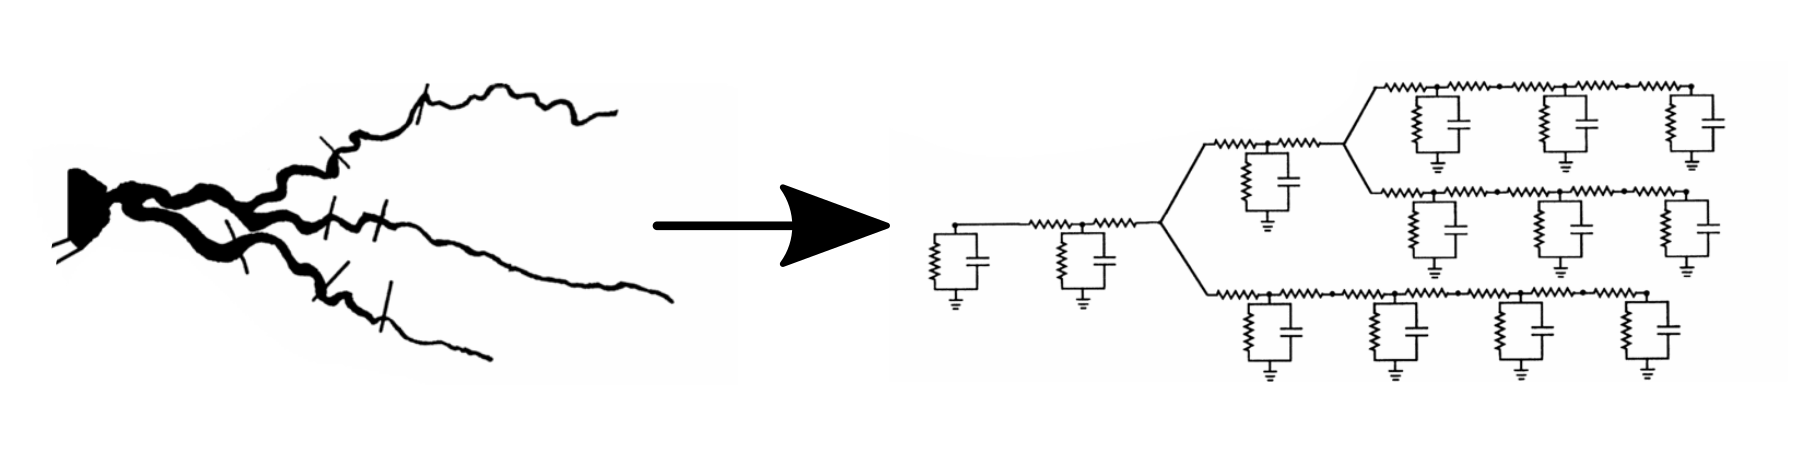
\includegraphics[width=1\textwidth]{model_creation.png}}
\end{figure}
\end{frame}


% \begin{frame}{Første modelen av et nevron ble laget av Hodgkin og Huxley i 1952}
%    \begin{figure}
%      \only<1>{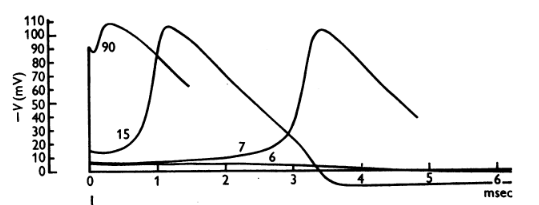
\includegraphics[width=1\textwidth]{original_hh.png}}
%      \only<2>{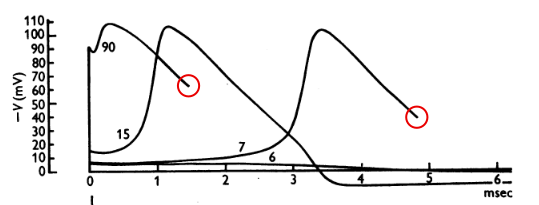
\includegraphics[width=1\textwidth]{original_hh2.png}}
%      \only<3>{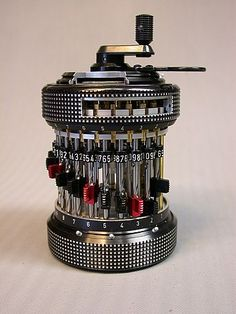
\includegraphics[width=0.4\textwidth]{calculator.jpg}}
% \end{figure}
% \end{frame}

\begin{frame}
    \begin{columns}
    \begin{column}{0.5\textwidth}
        \begin{center}
        \begin{figure}
            {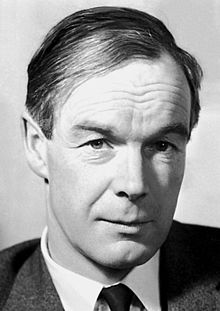
\includegraphics[width=1\textwidth]{hodgkin.jpg}}
            \caption*{Alan Lloyd Hodgkin}
     \end{figure}
    \end{center}
    \end{column}
    \begin{column}{0.5\textwidth}  %%<--- here
        \begin{center}
            \begin{figure}
                {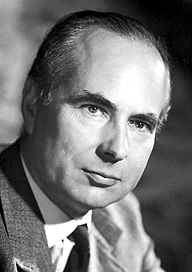
\includegraphics[width=1\textwidth]{huxley.jpg}}
                \caption*{Andrew Fielding Huxley}
         \end{figure}
         \end{center}
    \end{column}
    \end{columns}
\end{frame}



\begin{frame}
    \only<1>{\fullimage{original_hh.png}{0.8}}
    \only<2>{\fullimage{original_hh2.png}{0.8}}
\end{frame}

\begin{frame}
    {\fullimage{calculator.jpg}{0.8}}
\end{frame}

% \begin{frame}{Nevron modeller kan settes sammen til nettverk}
%    \begin{figure}
%      {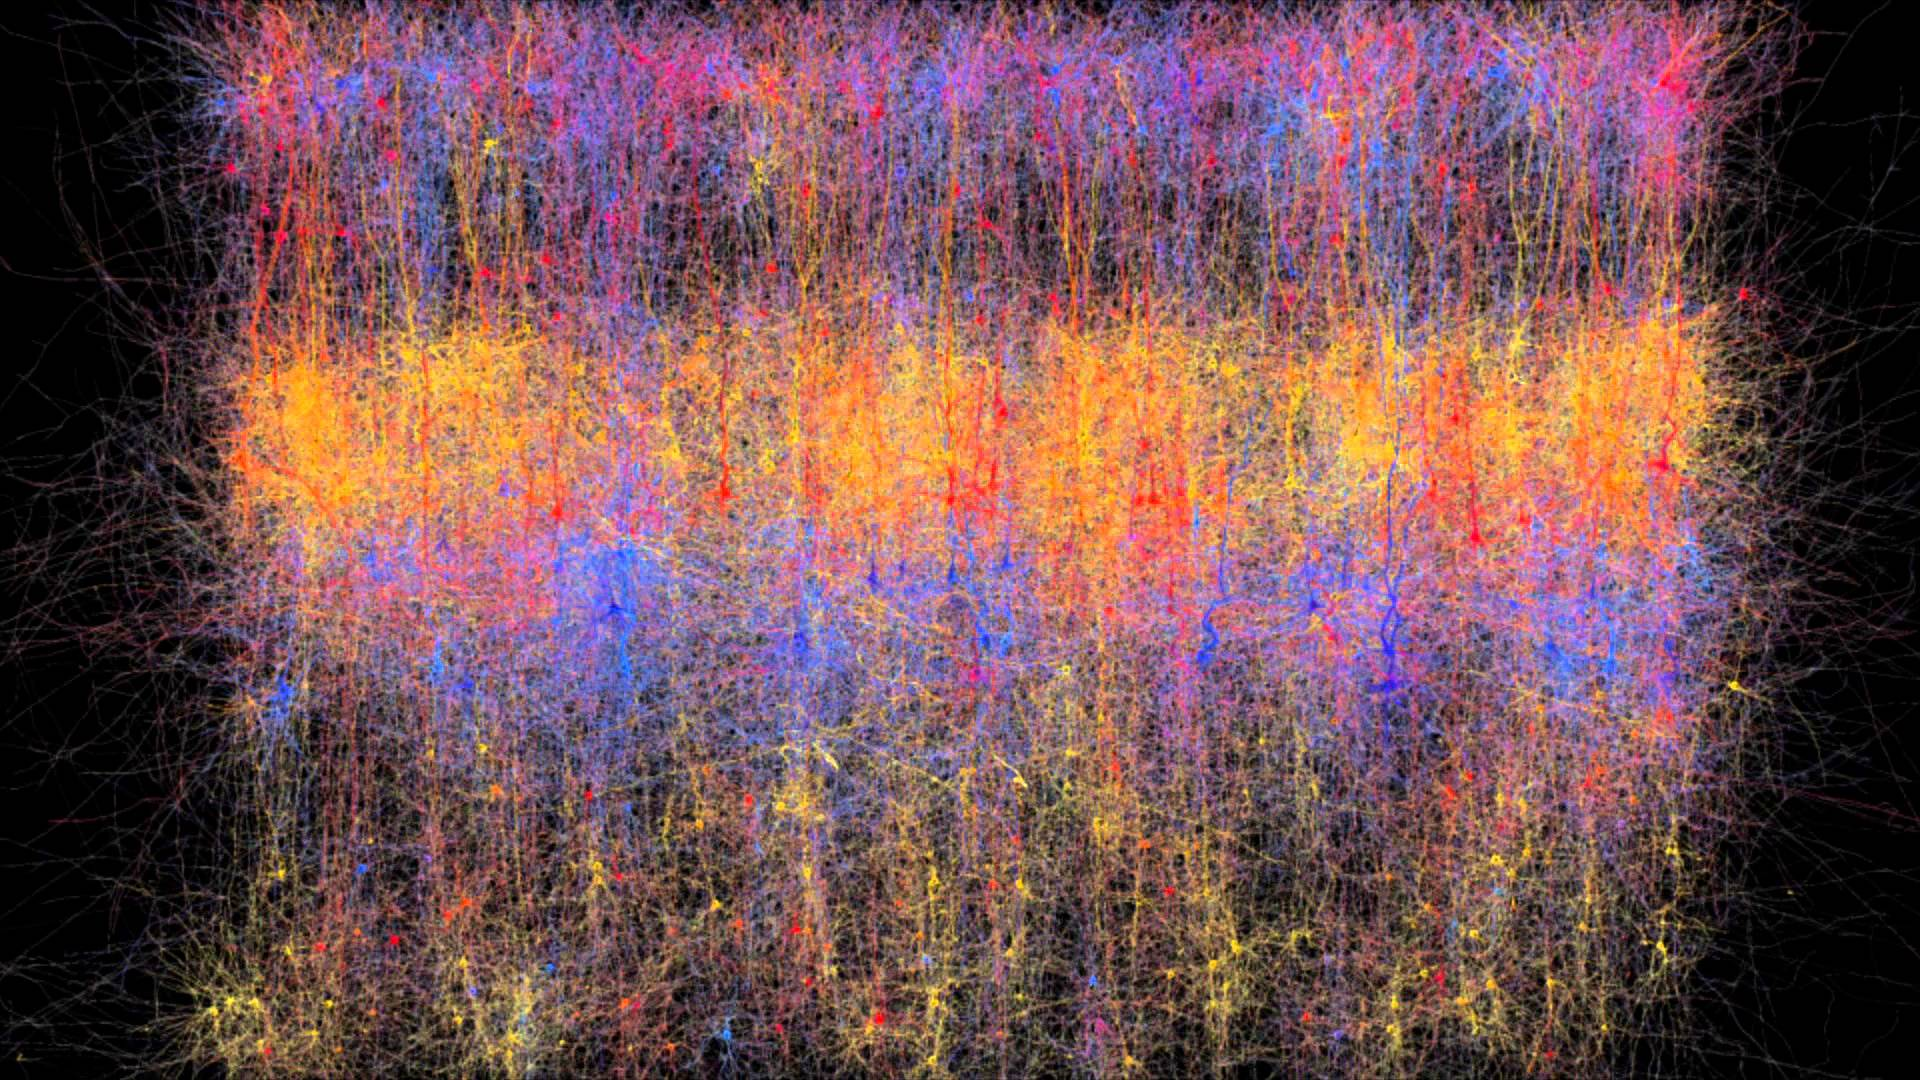
\includegraphics[width=1\textwidth]{network_large.jpg}}
% \end{figure}
% \end{frame}

\begin{frame}
    \fullimage{network_large.jpg}{.26}
\end{frame}


\begin{frame}{Realistiske nevroner krever tunge beregninger, i nettverk brukes derfor ofte enklere modeller}
\vspace{-10mm}
   \begin{figure}
       \only<1>{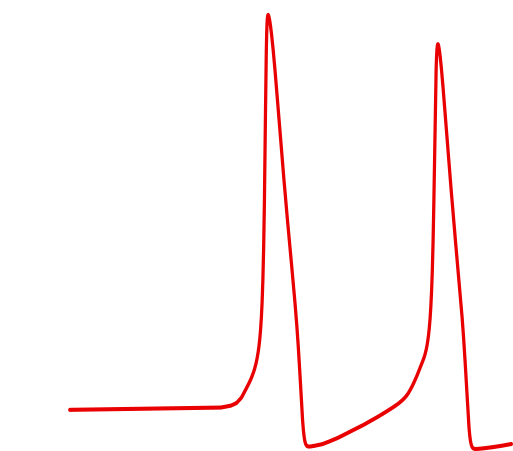
\includegraphics[width=.7\textwidth]{iaf_real.png}}
       \only<2>{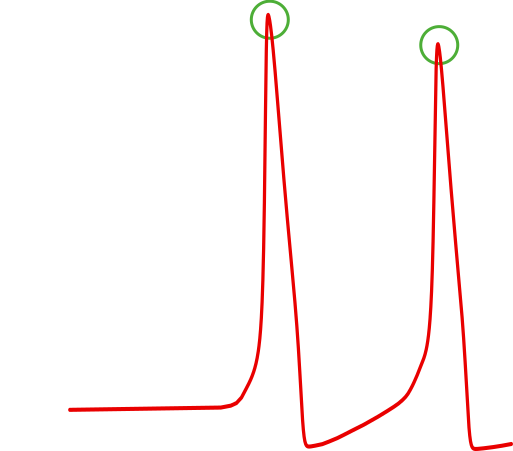
\includegraphics[width=.7\textwidth]{iaf_real_circle.png}}
     \only<3>{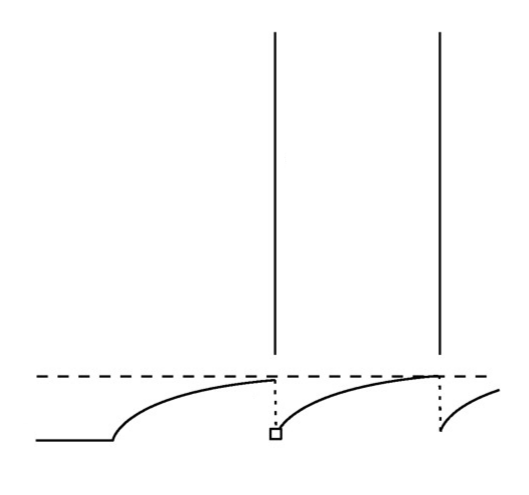
\includegraphics[width=.7\textwidth]{iaf.png}}
      \only<4>{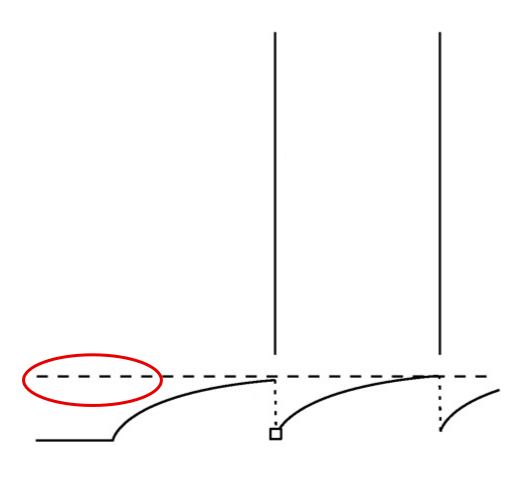
\includegraphics[width=.7\textwidth]{iaf_terskel.png}}
       \only<5>{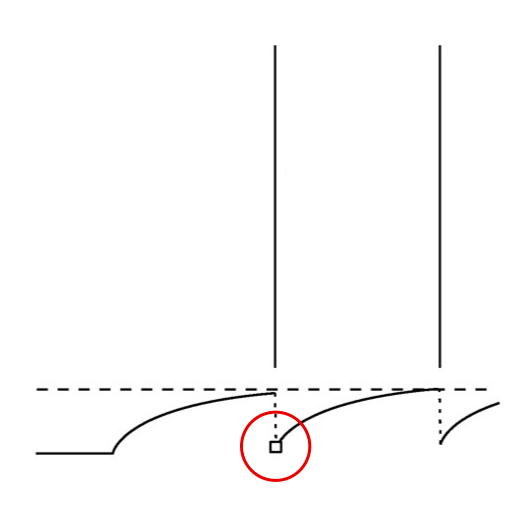
\includegraphics[width=.7\textwidth]{iaf_resatt.png}}
        \only<6>{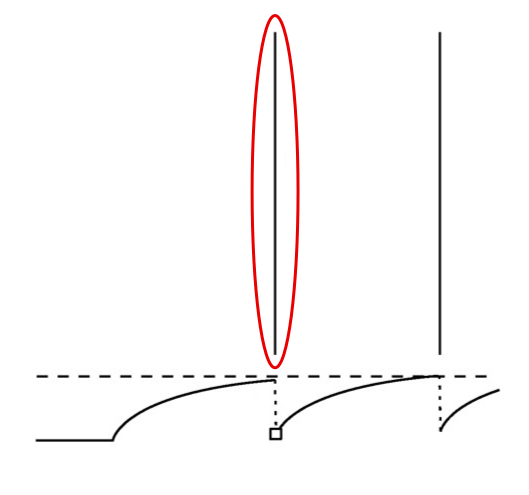
\includegraphics[width=.7\textwidth]{iaf_spike.png}}
\end{figure}
\end{frame}

% \begin{frame}{Neuronify lar dere lage realistiske netverk med enkle nevroner}
%    \begin{figure}
%      {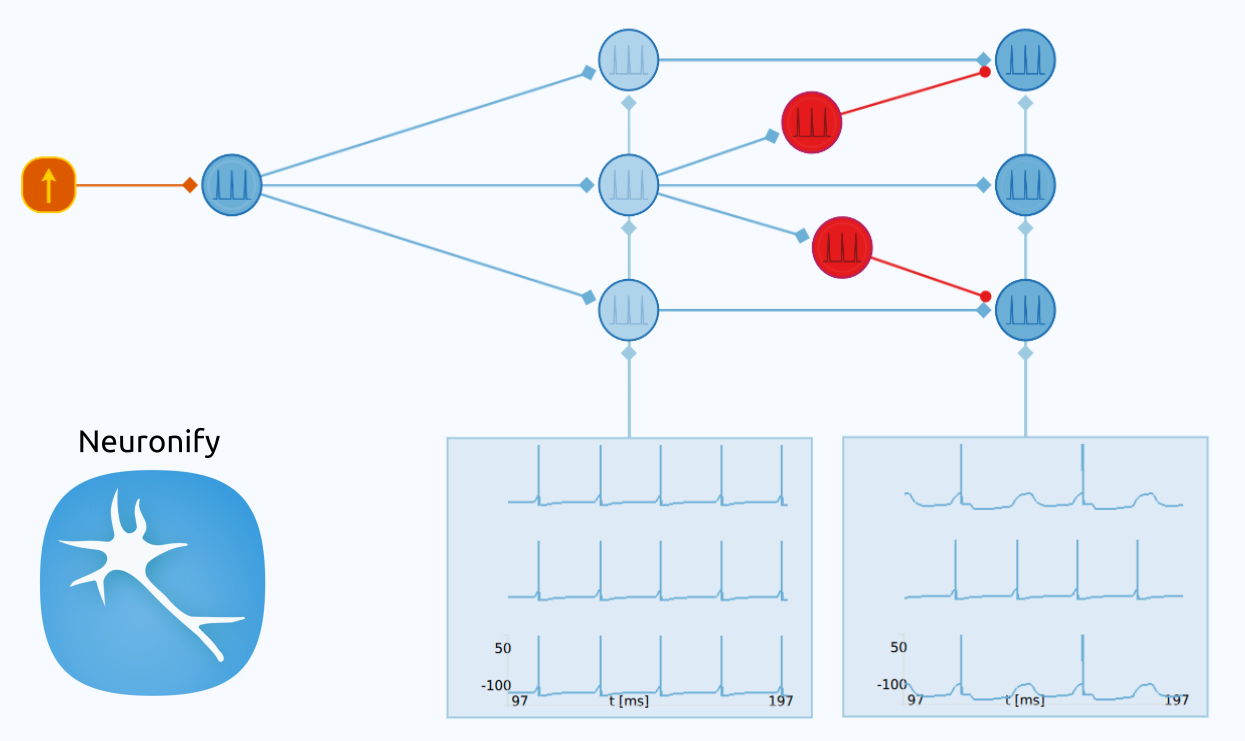
\includegraphics[width=1\textwidth]{neuronify_network.png}}
% \end{figure}
% \end{frame}



\begin{frame}
    \fullimage{neuronify_network.png}{.35}
\end{frame}


\begin{frame}[fragile]{}
    \begin{tikzpicture}[remember picture, overlay, font=\sffamily]
      \node [align=left, opacity=0.35, xshift=-0.4\textwidth,yshift=0.25\textwidth] (image3) at (current page.center)
            {\includegraphics[width = 0.2\textwidth]{brain.jpg}};
      \node[align=left, opacity=0.35] at (image3.east) {\hspace{6cm} \bf Grunnlegende nevrovitenskap};
    \end{tikzpicture}

  \begin{tikzpicture}[remember picture, overlay, font=\sffamily]
  \node [align=left, opacity=0.35, xshift=-0.2\textwidth,yshift=0\textwidth] (image1) at (current page.center)
      {\includegraphics[width = 0.2\textwidth]{brain_circuits.jpg}};
  \node[align=left, opacity=0.35] at (image1.east) {\hspace{7.5cm} \bf Beregningsorientert nevrovitenskap};
  \end{tikzpicture}


    \begin{tikzpicture}[remember picture, overlay, font=\sffamily]
      \node [align=left,  xshift=0\textwidth,yshift=-0.25\textwidth] (image2) at (current page.center)
            {\includegraphics[width = 0.2\textwidth]{logo_small.png}};
      \node[align=left] at (image2.east) {\hspace{4cm} \bf Usikkerhetsberegninger};
    \end{tikzpicture}
\end{frame}



\begin{frame}
    \fullimage{ap.png}{0.5}
\end{frame}




\begin{frame}{Forskjellige parametre gir forskjellige resultater}
        \begin{tikzpicture}[remember picture, overlay, font=\sffamily]
             \onslide<1-2>{\node [align=left, xshift=-0\textwidth, yshift=0.25\textwidth] (image3) at (current page.center)
                   {$I = C\frac{{\mathrm d} V}{{\mathrm d} t}  + I_{\text{kanaler}}$};}
               \onslide<3->{\node [align=left, xshift=-0\textwidth,yshift=0.25\textwidth] (image3) at (current page.center)
                     {$I = C\frac{{\mathrm d} V}{{\mathrm d} t}  + {\bf\color{logored}I_{\text{kanaler}}}$};}
           \end{tikzpicture}

           \begin{tikzpicture}[remember picture, overlay, font=\sffamily]
                \onslide<4>{\node [align=left, xshift=0\textwidth,yshift=-0.1\textwidth] (image3) at (current page.center)
                    {\includegraphics[width = 0.8\textwidth]{hh_variation.png}};}
                %   \node[align=left] at (image3.east) {\hspace{4cm} \bf Sette opp modellen};}
              \end{tikzpicture}

           \begin{tikzpicture}[remember picture, overlay, font=\sffamily]
                \onslide<2>{\node [align=left, xshift=0.3\textwidth,yshift=0.15\textwidth] (image3) at (current page.center)
                    {\includegraphics[width = 0.3\textwidth]{circuit2.png}};}
              \end{tikzpicture}
\end{frame}



% \begin{frame}%{Å lage en beregningsmodel består av tre steg, å sette opp modelen, estimere parametre og beregne usikkerhetene}
%     \begin{tikzpicture}[remember picture, overlay, font=\sffamily]
%       \onslide<1-3>{\node [align=left, xshift=-0.35\textwidth,yshift=0.25\textwidth] (image3) at (current page.center)
%             {$I = C\frac{{\mathrm d} V}{{\mathrm d} t}  + I_{\text{kanaler}}$};
%       \node[align=left] at (image3.east) {\hspace{4cm} \bf Sette opp modellen};}
%     \end{tikzpicture}
%    %
%    % \begin{tikzpicture}[remember picture, overlay, font=\sffamily]
%    %   \onslide<1-3>{\node [align=left, xshift=-0.4\textwidth,yshift=0.15\textwidth] (image3) at (current page.center)
%    %         {\includegraphics[width = 0.4\textwidth]{compartmental.png}};
%    %   \node[align=left] at (image3.east) {\hspace{5cm} \bf Model creation};}
%    % \end{tikzpicture}
%
%   \begin{tikzpicture}[remember picture, overlay, font=\sffamily]
%   \onslide<2-3>{\node [align=left, xshift=-0.2\textwidth,yshift=-0.0\textwidth] (image1) at (current page.center)
%       {\includegraphics[width = 0.15\textwidth]{parameters.png}};
%   \node[align=left] at (image1.east) {\hspace{4.5cm} \bf Parameter estimering};}
%   \end{tikzpicture}
%
%     \begin{tikzpicture}[remember picture, overlay, font=\sffamily]
%       \onslide<3-4>{\node [align=left, xshift=0\textwidth,yshift=-0.25\textwidth] (image2) at (current page.center)
%             {\includegraphics[width = 0.25\textwidth]{confidence_interval.png}};
%       \node[align=left] at (image2.east) {\hspace{4cm} \bf Usikkerhetsberegning};}
%     \end{tikzpicture}
%
% \end{frame}






% \begin{frame}{Problem: Experimental measurements always contain errors}
%     \begin{figure}
%         \includegraphics[width=1\textwidth]{dist.png}
%     \end{figure}
% \end{frame}

% \begin{frame}{Tradisjonelle modeller er deterministiske}
%     \begin{figure}
%       %  \only<1>{\includegraphics[width=0.6\textwidth]{model2.png}}
%        \includegraphics[width=1.1\textwidth]{deterministic.png}
%
%     \end{figure}
% \end{frame}

\begin{frame}
    \only<1>{\fullimage{deterministic_model.png}{.45}}
    \only<2>{\fullimage{deterministic_input.png}{.45}}
    \only<3>{\fullimage{deterministic.png}{.45}}
\end{frame}


% \begin{frame}{Problemet er at biologiske parametre ikke er fiksert, men varierer}
%         \vspace{-1cm}
%     \begin{figure}
% \includegraphics[width=1\textwidth]{distributions.png}
% \end{figure}
% \end{frame}

\begin{frame}
    {\fullimage{distributions.png}{.25}}
\end{frame}



% \begin{frame}{Løsningen er å gjøre en usikkerhetsberegning}
%         \vspace{-1cm}
%     \begin{figure}
%       %  \only<1>{\includegraphics[width=0.6\textwidth]{model2.png}}
%        {\includegraphics[width=1.1\textwidth]{probabalistic_no_uncertainpy.png}}
%
%     \end{figure}
% \end{frame}

% \begin{frame}{Min forskning går ut på å lage software for å gjøre disse usikkerhetsberegningene}
%     \vspace{-1cm}
%     \begin{figure}
%       %  \only<1>{\includegraphics[width=0.6\textwidth]{model2.png}}
%        {\includegraphics[width=1.1\textwidth]{probabalistic.png}}
%
%     \end{figure}
% \end{frame}


\begin{frame}
    \only<1>{\fullimage{probabalistic_no_uncertainpy.png}{.35}}
    \only<2>{\fullimage{probabalistic.png}{.35}}
\end{frame}


% \begin{frame}{Uncertainty quantification relates uncertain parameters and model results}
%     \begin{figure}
%         \only<1>{\includegraphics[width=0.5\textwidth]{model1.png}}
%         \only<2>{\includegraphics[width=0.5\textwidth]{model2.png}}
%         \only<3>{\includegraphics[width=0.5\textwidth]{model3.png}}
%         \only<4>{\includegraphics[width=0.5\textwidth]{model4.png}}
%     \end{figure}
% \end{frame}





















% \begin{frame}{Uncertainty quantification relates measurements errors and model results}
% % \begin{itemize}
% %     \item accuracy of model
% %     \item effect of uncertain input
% %     \item relationship between uncertain input and output
% %
% % \end{itemize}
% \end{frame}
%\begin{frame}
%    \begin{center}
%        {\usebeamercolor[fg]{frametitle} \Large \bf UncertainPy performs these calculations}
%    \end{center}
%\end{frame}


% \begin{frame}{Monte Carlo metoder simulerer mange eksperimenter på en model, som så kan gjøre statistikk på resultatene fra}
%    \vspace{-5mm}
% \begin{figure}
%     \only<1>{\includegraphics[width=1.1\textwidth]{mc.png}}
%     \only<2>{\includegraphics[width=1.1\textwidth]{mc_1-1.png}}
%     \only<3>{\includegraphics[width=1.1\textwidth]{mc_1-2.png}}
%     \only<4>{\includegraphics[width=1.1\textwidth]{mc_1-3.png}}
%     \only<5>{\includegraphics[width=1.1\textwidth]{mc_2.png}}
%     \only<6>{\includegraphics[width=1.1\textwidth]{mc_3.png}}
% \end{figure}
% \end{frame}



\begin{frame}
    \only<1>{\fullimage{casino.jpg}{.7}}
\end{frame}


\begin{frame}
    \only<1>{\fullimage{mc.png}{.35}}
    \only<2>{\fullimage{mc_1-1.png}{.35}}
    \only<3>{\fullimage{mc_1-2.png}{.35}}
    \only<4>{\fullimage{mc_1-3.png}{.35}}
    \only<5>{\fullimage{mc_2.png}{.35}}
    \only<6>{\fullimage{mc_3.png}{.35}}
\end{frame}




\begin{frame}{Resultat: Usikkerhet i aksjonspotensialet \\(90\% konfidensintervall)}
   \vspace{-5mm}
\begin{figure}
   \only<1>{\includegraphics[width=0.8\textwidth]{confidence_interval.png}}
   \only<2>{\includegraphics[width=0.8\textwidth]{confidence_interval_arrow.png}}
\end{figure}
\end{frame}



% \begin{frame}{\onslide<1->{Punktvis sammenligning \onslide<2->{er problematisk siden "samme" aksjonspotensial kan komme til forskjellige tider med forskjellige parametre}}}
%    \vspace{-5mm}
%    \begin{figure}
%     %   \only<1>{\includegraphics[width=1\textwidth]{hh_basic.png}}
%       \only<1>{\includegraphics[width=0.8\textwidth]{hh_pointwise.png}}
%       \only<2>{\includegraphics[width=0.8\textwidth]{hh_arrows.png}}
%    \end{figure}
% \end{frame}

% \begin{frame}{90\% confidence interval for the Hodgkin-Huxley model with original uncertainties in the parameters}
%    \vspace{-5mm}
% \begin{figure}
%    \only<1>{\includegraphics[width=0.8\textwidth]{confidence-interval.png}}
%    \only<2>{\includegraphics[width=0.8\textwidth]{confidence-interval_elipse.png}}
% \end{figure}
% \end{frame}


% \begin{frame}{Løsningen er å jobbe med egenskaper til nevronet slik som antall aksjonspotensialer{\color{white} dummy text dummy text dummy text dummy text dummy text} }
% \vspace{-5mm}
% \begin{figure}
%    \includegraphics[width=0.8\textwidth]{hh_features.png}
% \end{figure}
% \end{frame}

% \begin{frame}{UncertainPy calculates the uncertainty for features such as the number of spikes}
% \vspace{-5mm}
% \begin{figure}
%    \includegraphics[width=0.65\textwidth]{features.png}
% \end{figure}
% \end{frame}


% \begin{frame}{Sensitivity of the result for each parameter in the Hodgkin-Huxley model}
% \vspace{-5mm}
% \begin{figure}
%    \includegraphics[width=1\textwidth]{sensitivity_grid.png}
% \end{figure}
% \end{frame}

% \begin{frame}{UncertainPy is model independent}
%     \begin{center}
% \begin{figure}
%         \begin{minipage}[b]{0.45\linewidth}
%             \centering
%             \includegraphics[width=\textwidth]{nest.png}
%             \caption*{Raster plot of excitatory neurons in a Brunel network}
%         \end{minipage}
%         \hspace{0.5cm}
%         \begin{minipage}[b]{0.45\linewidth}
%             \centering
%             \includegraphics[width=\textwidth]{nest_result.png}
%             \caption*{Mean coefficient of variation}
%         \end{minipage}
%     \end{figure}
% \vspace{2cm}
% \end{center}
% \end{frame}



  \begin{frame}{Oppsumering: beregningsorientert nevrovitenskap modelerer nevroner som elektriske kretser}
\vspace{-15mm}
\begin{columns}

     \column{.5\textwidth}
     \begin{center}
        \raggedright
      \bf{Nevroner kan modeleres som elektriske kretser i ett nettverk}
     \end{center}
     \column{.5\textwidth}
     \begin{center}
            \includegraphics[width=0.4\textwidth]{circuit2.png}
     \end{center}

 \end{columns}

 % \vspace{5mm}
\pause
\begin{columns}
  \column{.5\textwidth}
  \begin{center}
      \raggedright
   \bf{Usikkerhetsberegninger gjør at man kan ta hensyn til biologiske parametre som varierer}
  \end{center}
       \column{.5\textwidth}
     \begin{center}
            \includegraphics[width=0.9\textwidth]{probabalistic_no_uncertainpy.png}
     \end{center}

 \end{columns}


  %  \begin{tikzpicture}[remember picture, overlay, font=\sffamily]
  %      \node [align=left, xshift=0.49\textwidth,yshift=-0.37\textwidth] (image2) at (current page.center)
  %            {\includegraphics[width = 0.3\textwidth]{cinpla.png}};
  %    \end{tikzpicture}


\pause
\begin{tikzpicture}[remember picture, overlay, font=\sffamily]

  \node[align=left, yshift=0.1\textwidth, opacity=0.9] at (current page.south){ \bf \large Takk for meg!};
\end{tikzpicture}



\end{frame}


\end{document}
\grid
